\section{Probability Mass on Incorrect Choices Causes Unpredictability}

\begin{figure*}[t!]
    \centering
    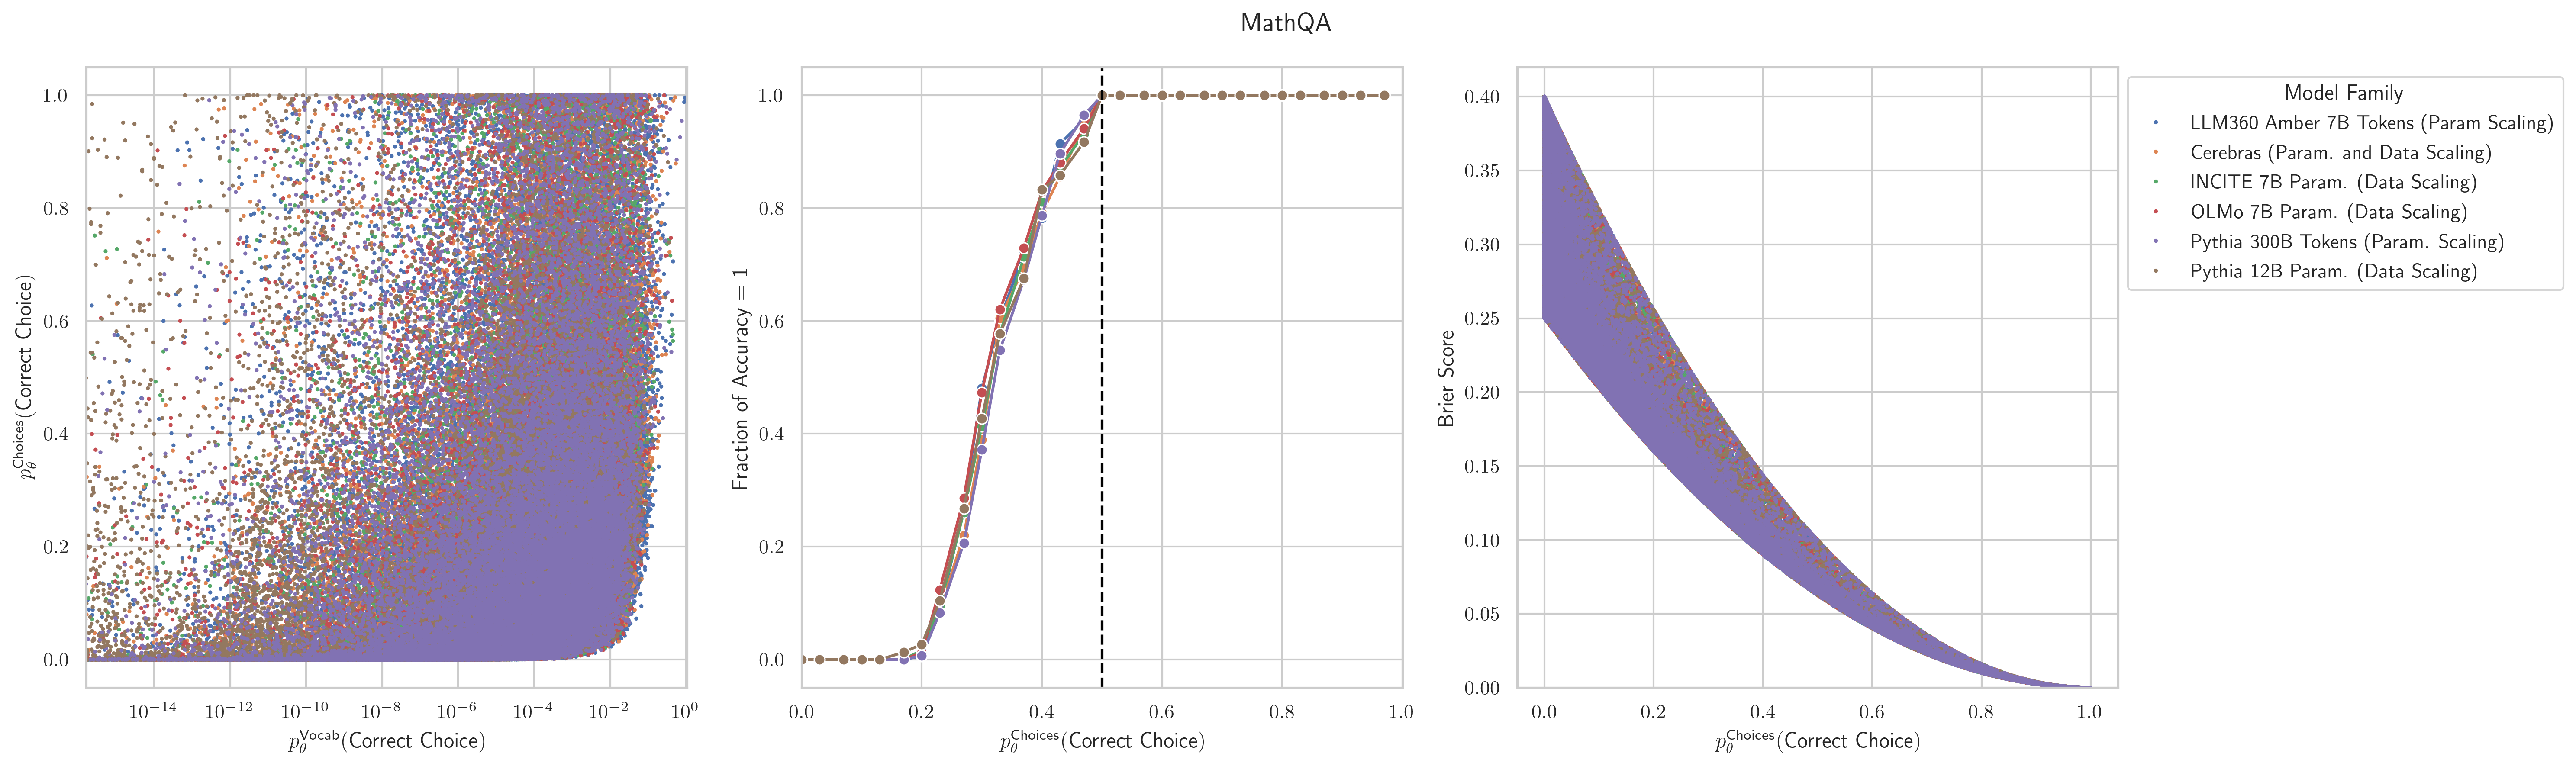
\includegraphics[width=\textwidth]{figures/pairwise_metric_comparisons/mathqa/mathqa_p_choices_corr_vs_p_vocab_corr_and_acc_vs_p_choices_corr_and_brier_score_vs_p_choices_corr_by_model_family.png}
    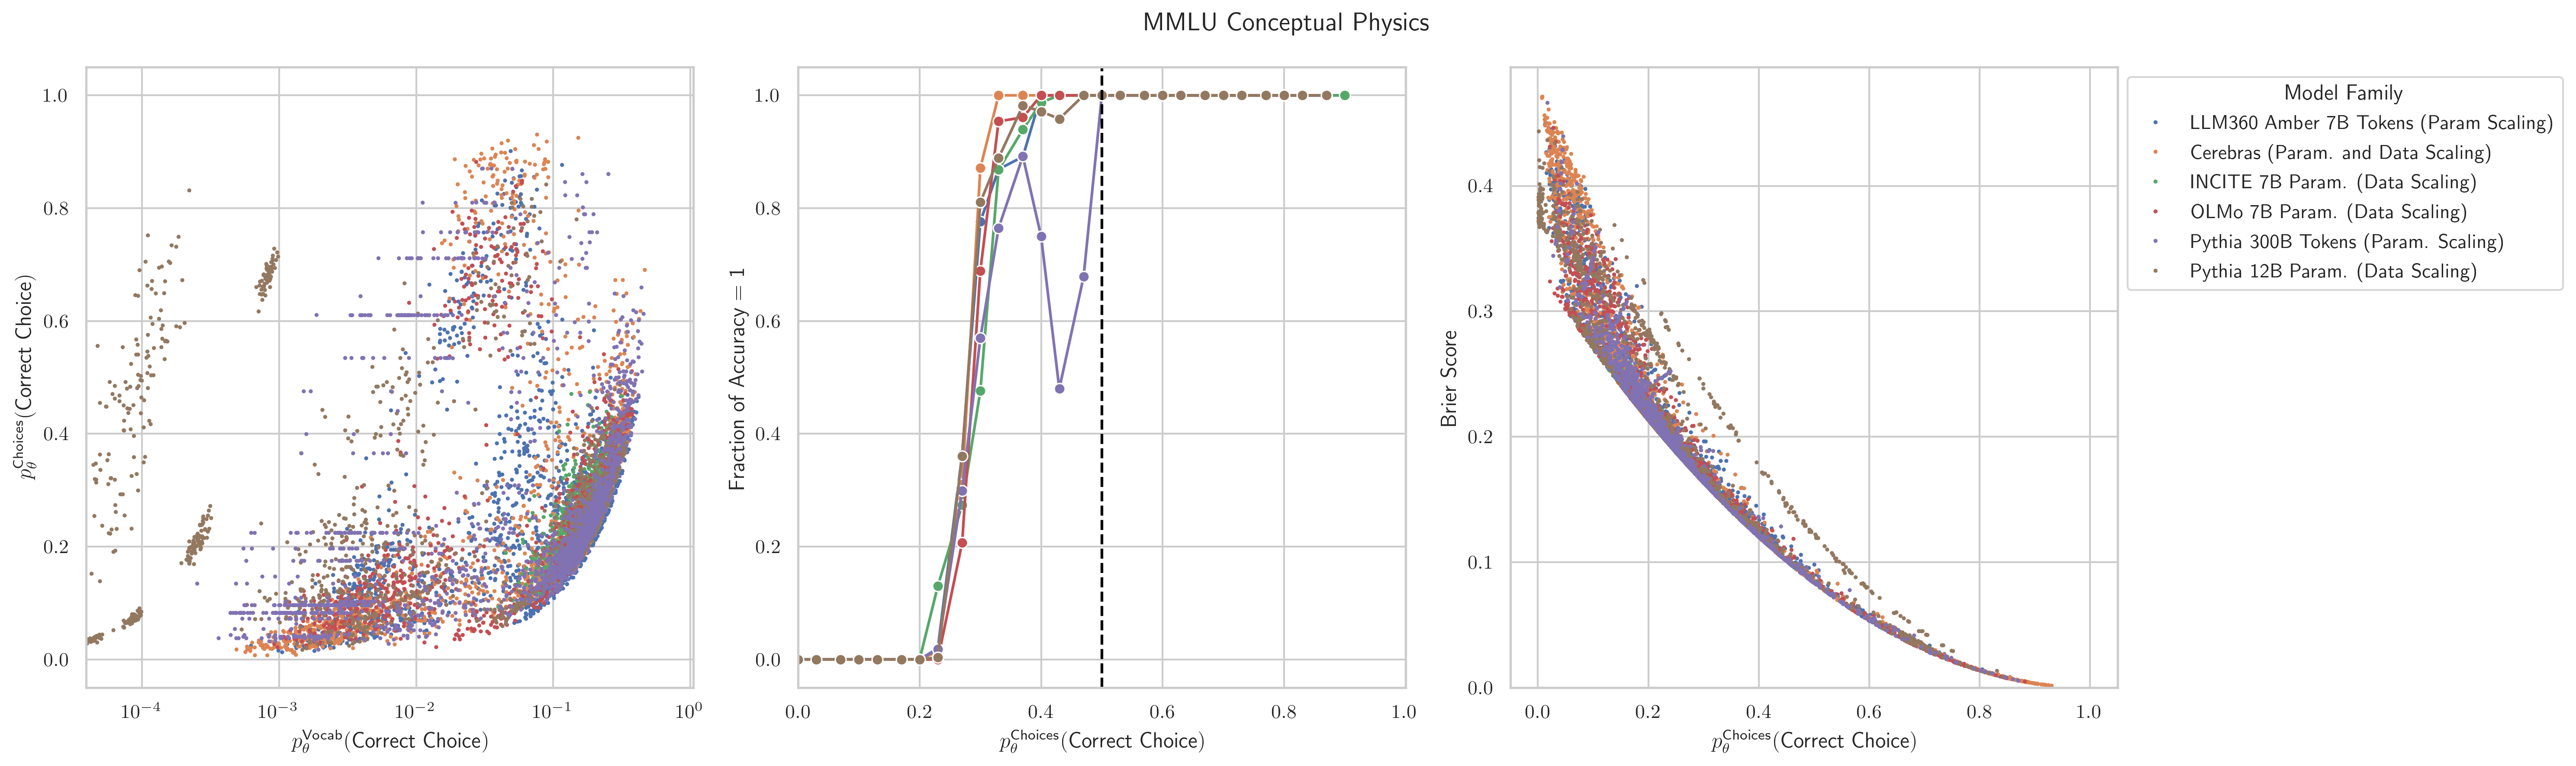
\includegraphics[width=\textwidth]{figures/pairwise_metric_comparisons/mmlu_conceptual_physics/mmlu_conceptual_physics_p_choices_corr_vs_p_vocab_corr_and_acc_vs_p_choices_corr_and_brier_score_vs_p_choices_corr_by_model_family_scatter.png}
    % 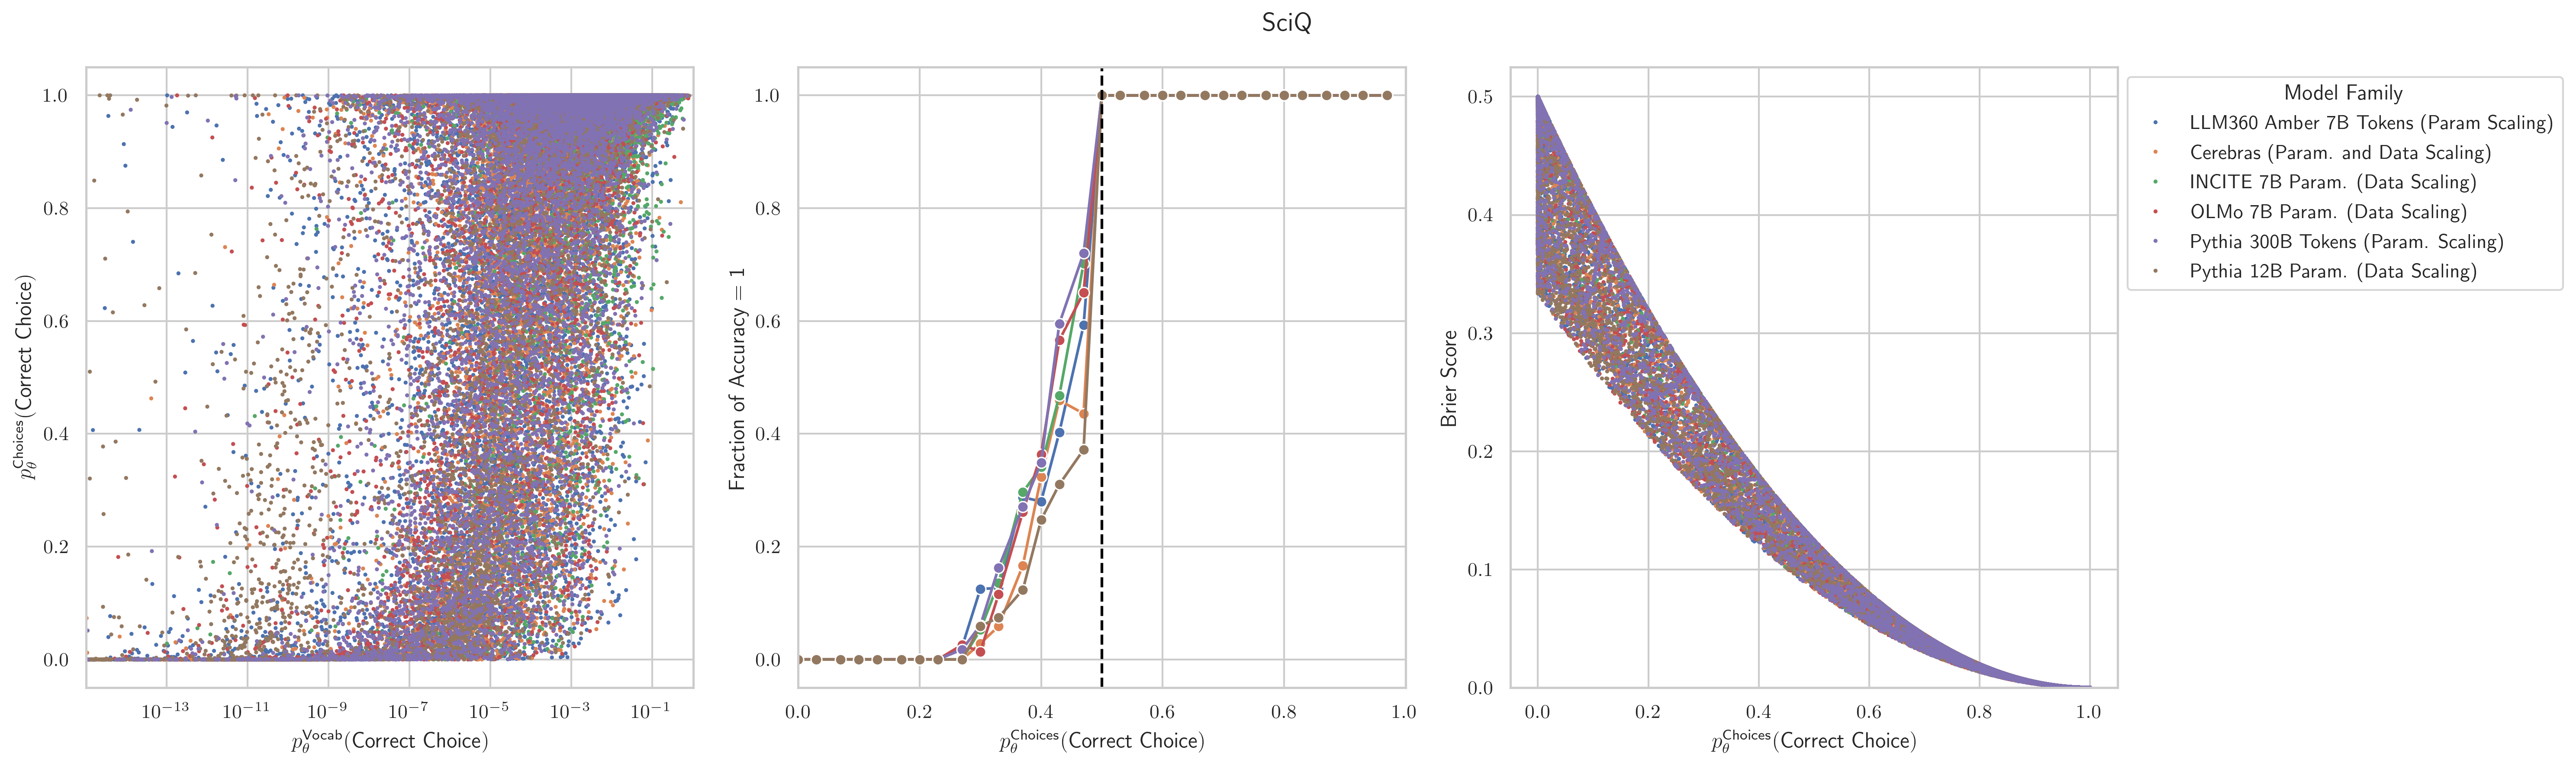
\includegraphics[width=\textwidth]{figures/pairwise_metric_comparisons/sciq/sciq_p_choices_corr_vs_p_vocab_corr_and_acc_vs_p_choices_corr_and_brier_score_vs_p_choices_corr_by_model_family_scatter.png}
    \caption{\textbf{Predictability deteriorates because of probability mass fluctuating on alternative incorrect choices with scale.} \textbf{Left:} Transitioning from $p_{\theta}^{\text{Vocab}}(\text{Correct Choice})$ to $p_{\theta}^{\text{Choices}}(\text{Correct Choice})$ demonstrates that $p_{\theta}^{\text{Vocab}}(\text{Correct Choice})$ contains little information about $p_{\theta}^{\text{Choices}}(\text{Correct Choice})$ and vice versa; loosely speaking, any value of one can map to any value of the other. \textbf{Center:} While $p_{\theta}^{\text{Choices}}(\text{Correct Choice}) > 0.5$ must yield $\texttt{Accuracy} = 1$, for any $p_{\theta}^{\text{Choices}}(\text{Correct Choice}) < 0.5$, knowing $p_{\theta}^{\text{Choices}}(\text{Correct Choice})$ contains little information about $\texttt{Accuracy}$ and vice versa. \textbf{Right}: \texttt{Brier Score} is more predictable from $p_{\theta}^{\text{Choices}}(\text{Correct Choice})$ than \texttt{Accuracy}, but still quite variable. Two benchmarks shown: MathQA \& MMLU Conceptual Physics.%, SciQ \cite{welbl2017sciq}.
    }
    \label{fig:pairwise_metric_comparisons}
\end{figure*}

What is the mechanism that degrades how scores correlate with compute? All three metrics with degraded correlations - $p_{\theta}^{\text{Choices}}(\text{Correct Choice})$, \texttt{Accuracy}, and \texttt{Brier Score} - depend not just on how the model's probability mass $p_{\theta}^{\text{Vocab}}(\text{Correct Choice})$ concentrates on the correct choice as compute increases, but also depend on how the model's probability mass fluctuates on \textit{incorrect} available choices $\{ p_{\theta}^{\text{Vocab}}(\text{Incorrect Choice}) \}_{\text{Incorrect Choices}}$ as compute increases. As an example, suppose $p_{\theta}^{Vocab}(\text{Correct Choice}) = 0.4$ on a 4-way multiple-choice question; what is the accuracy? Spreading the remaining mass uniformly on the incorrect choices will make \texttt{Accuracy} $=1$, whereas concentrating mass on a single incorrect choice will make \texttt{Accuracy} $=0$.




To demonstrate how drastically the probability mass placed on incorrect choices can alter performance, we visualized the relationships between pairs of metrics immediately preceding and following a given transformation (Fig. \ref{fig:pairwise_metric_comparisons}). For negative log likelihood of the correct choice and $p_{\theta}^{Vocab}(\text{Correct Choice})$ (not pictured), we observed a clean correspondence between performance under the metric and compute: one can reliably map a given value of these metrics to compute, and vice versa. In contrast, once performance is evaluated using a metric that is a function of the incorrect choices - $p_{\theta}^{\text{Choices}}(\text{Correct Choice})$, \texttt{Accuracy} or \texttt{Brier Score} - nearly any value of a score under one metric can map to any value of $p_{\theta}^{\text{Vocab}}(\text{Correct Choice})$ or $p_{\theta}^{\text{Choices}}(\text{Correct Choice})$ respectively (Fig. \ref{fig:pairwise_metric_comparisons}), thereby breaking the chain along which one can cleanly infer compute from an observed metric. We can see that \texttt{Brier Score}, a metric meant to produce more continuous scores \citep{schaeffer2023mirage}, is less variable than \texttt{Accuracy}, provided a known $p_{\theta}^{\text{Choices}}(\text{Correct Choice})$, but it cannot recover information about $p_{\theta}^{\text{Vocab}}(\text{Correct Choice})$ that is lost when shifting to $p_{\theta}^{\text{Choices}}(\text{Correct Choice})$. We next show that this is because of the additional information regarding the underdetermined values of $p_{\theta}^{\text{Choices}}(\text{Incorrect Choice})$ for each incorrect choice.